\section{Visual analytics workflow}
\label{sec:workflow}

Figure~\ref{fig:master-workflow} follows the visual analytics process of
Keim et~al.~\cite{keim2008}. Following a strand shows what data went
into a model, what the analyst inspected, and which observation motivated a
change. The edge labelled \emph{Feedback loop} connects the first
inference to the transformation. The second set of models and views then
shows what changed.

The three analysts use the fixed split from Section~\ref{sec:a3-prep} for
different questions. Tushaar clusters students by their habits, checks how
the clusters differ in prior attainment and exam scores, then fits fresh
models within each prior-GPA band. Advaya's classification strand examines
how well the dropout flag can be recovered after removing the inputs that
define it. Aman's regression strand examines how the score ceiling and
prior attainment change the interpretation of background variables and
tutoring. The common identifiers, outcome definitions and split allow the
team to compare these findings.

\begin{figure}[H]
  \centering
  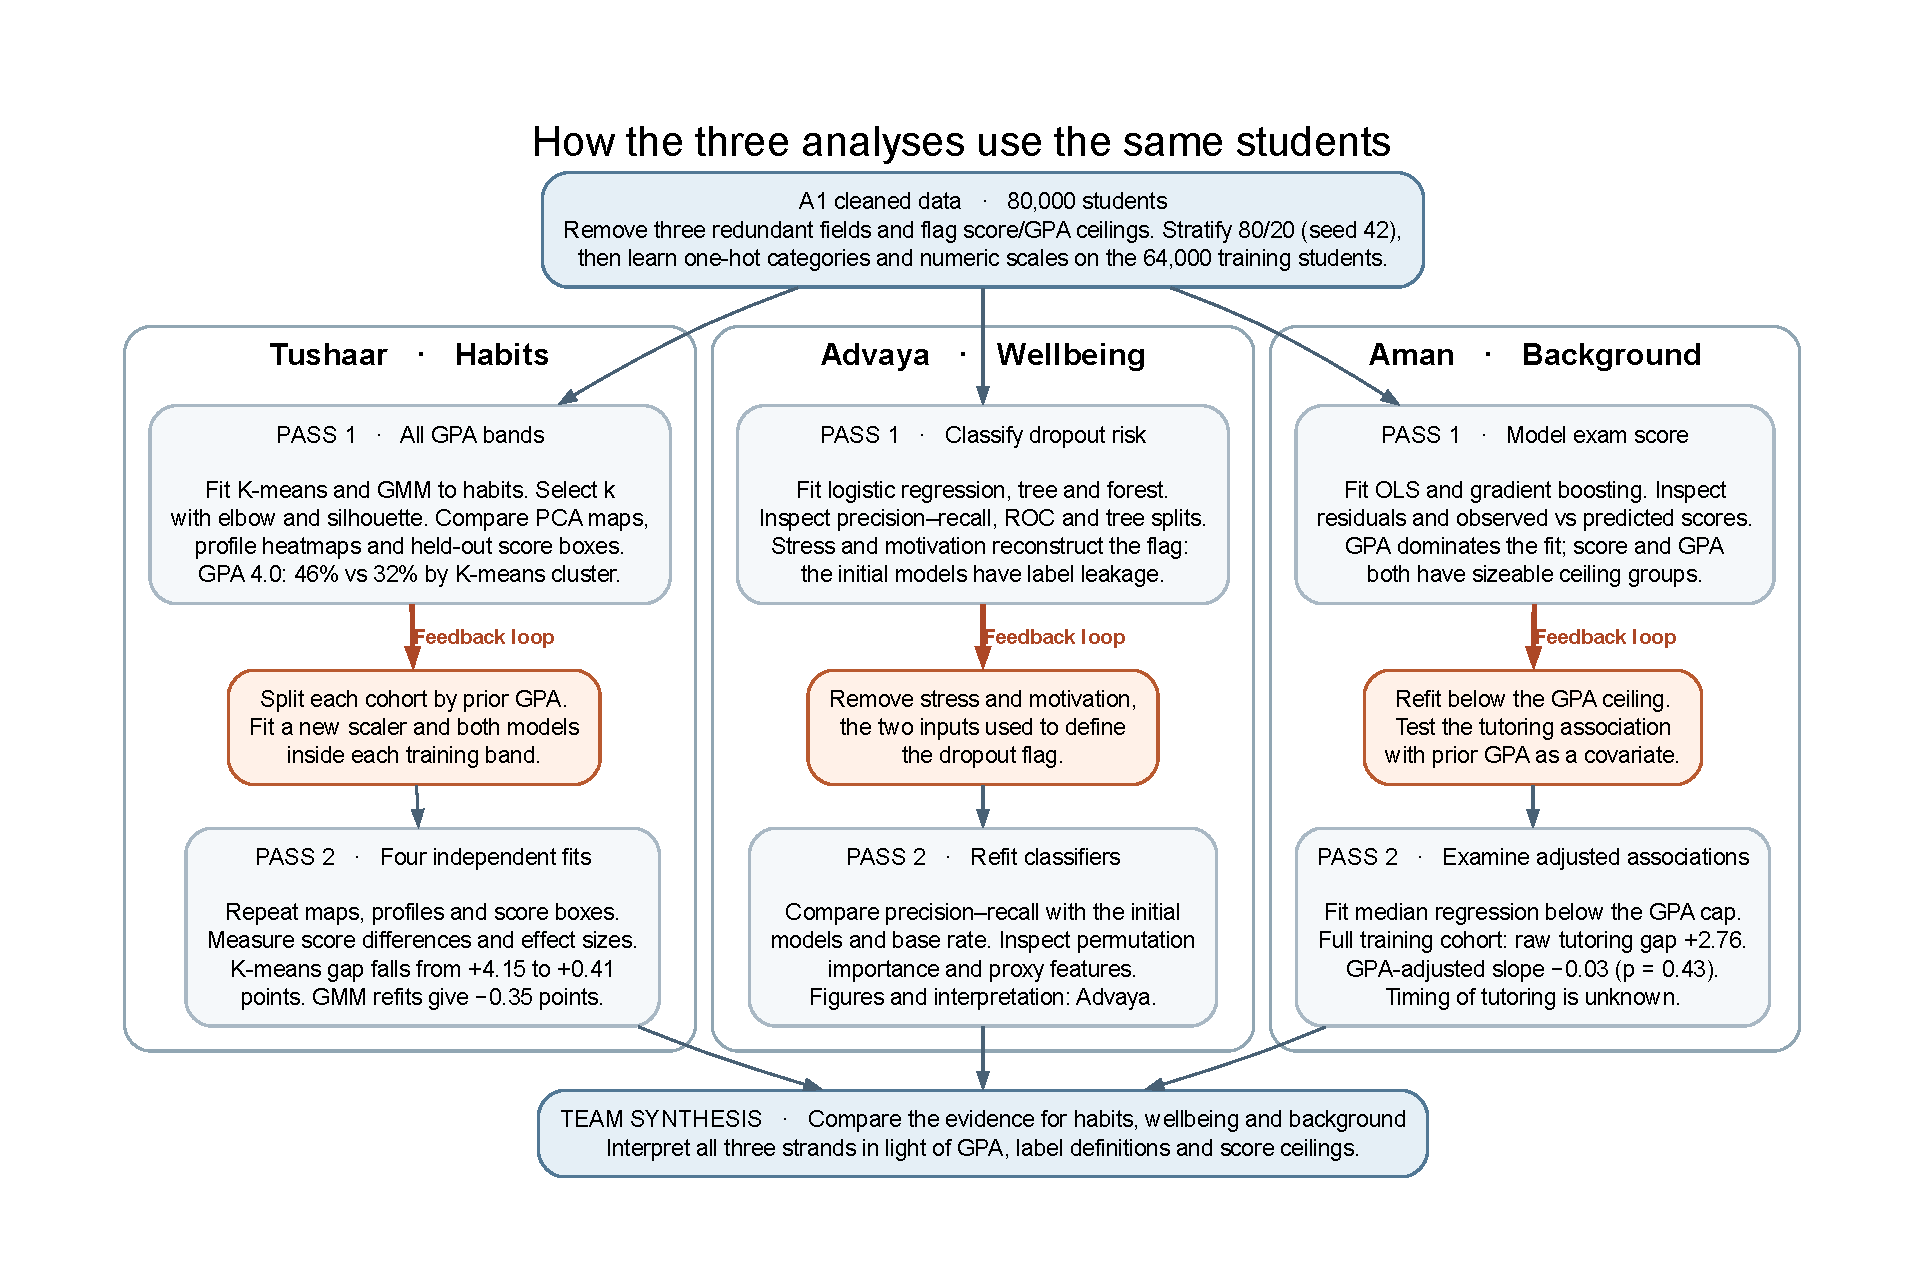
\includegraphics[width=\textwidth,height=.37\textheight,keepaspectratio]{diagrams/A3_master_workflow.pdf}
  \caption{The shared A3 workflow. Each column unrolls one analyst's two
  iterations. The labelled edge records the inference that changes the
  next analysis.}
  \label{fig:master-workflow}
\end{figure}
